\documentclass{article}

%%% Fill details here (in the second brackets)
\newcommand{\name}{Chris Bonney}     % Your name (First Last)
\newcommand{\wustlkey}{crbonney}             % Your WUSTL Key
%%%



%%%%%%%%%%%%%%%%%%%%%% Formatting Stuff %%%%%%%%%%%%%%%%%%%%%%%%%%%
\usepackage{times}
\usepackage[T1]{fontenc}

\setlength{\parskip}{1em}\setlength{\parindent}{0pt}
\linespread{1.25}
\usepackage[margin=0.7in,top=1in]{geometry}\usepackage{fancyhdr}
\pagestyle{fancy}\lhead{\bf \name}\rhead{\bf \wustlkey}\cfoot{\thepage}
\newcommand{\info}{\clearpage \subsection*{Information}}
\newcommand{\solution}[1]{\clearpage \subsection*{Solution #1}}
\newcommand{\spart}[1]{\paragraph{(#1)}}
%%%%%%%%%%%%%%%%%%%%%%%%%%%%%%%%%%%%%%%%%%%%%%%%%%%%%%%%%%%%%%%%%%%


%%% Add any more packages if you want to
\usepackage{amsmath,graphicx}
\graphicspath{{code/outputs/}}


\begin{document}
%%%%% Main Body goes here

% Begin solution to every problem like this.
\solution{1} 

\spart{a} To find the minimum over $x$ of 
\begin{align}
	f(x) = (x-y)^2+\lambda|x|
\end{align}
we start by proving that $f(x)$ is a convex function over $\mathcal{R}$ for $\lambda\geq0$. To do this, we will use a theorem, $f(x)$ is convex iff 
\begin{align}
	f(a) \geq f(b) + \partial f(b)(a-b) \quad \forall x,y \in \mathcal{R}
\end{align}
where $\partial f$ is defined to be the subgradient of $f$. To start, we compute the subgradient of the non-differentiable function:
\begin{align}
	\partial f(x) = 2(x-y) + \begin{cases}
		\lambda \quad &\text{for} \quad x>0 \\
		\lambda [-1,1] \quad &\text{for} \quad  x=0 \\
		-\lambda \quad &\text{for} \quad  x>0
	\end{cases} 
\end{align}
We then plug this in to the theorem above, and show that it holds. We get
\begin{align}
	(a-y)^2+\lambda|a| \geq (b-y)^2+\lambda|b| + 2(b-y)(a-b) + (a-b) \begin{cases}
		\lambda \quad &\text{for} \quad b>0 \\
		\lambda [-1,1] \quad &\text{for} \quad  b=0 \\
		-\lambda \quad &\text{for} \quad  b>0
	\end{cases} 
\end{align}
Rearranging, and canceling terms we simplify it to
\begin{align}
	(a-b)^2+\lambda(|a|-|b|) \geq \begin{cases}
	\lambda(a-b) \quad &\text{for} \quad b>0 \\
	\lambda a [-1,1] \quad &\text{for} \quad  b=0 \\
	-\lambda (a-b) \quad &\text{for} \quad  b>0
\end{cases} 
\end{align}
Considering each case individually, we get three inequalities that must hold: 
\begin{align}
	(a-b)^2+\lambda(|a|-|b|) &\geq \lambda(a-b) \quad \text{for} \quad b>0\\
	(a-b)^2+\lambda(|a|-|b|) &\geq \lambda a [-1,1] \quad \text{for} \quad b=0\\
	(a-b)^2+\lambda(|a|-|b|) &\geq -\lambda(a-b) \quad \text{for} \quad b<0
\end{align}
For the first inequality, we rewrite it as 
\begin{align}
	(a-b)^2+\lambda(|a|-a) - \lambda(|b|-b) &\geq 0 \quad \text{for} \quad b>0
\end{align}
and note that every term is greater than or equal to zero. The absolute value of a scalar subtracted by itself can be
\begin{align}
	|a|-a = \begin{cases}
		0 \quad &\text{for} \quad a \geq 0 \\
		-2a \quad &\text{for} \quad a<0
		\end{cases}
\end{align}
Since we assume $b>0$, $|b|-b = 0$, and $|a|-a\geq 0$ for any $a$, the inequality holds. For the second case, we simply set $b=0$ for all terms to get
\begin{align}
	(a)^2+\lambda(|a|-a[-1,1]) &\geq 0 
\end{align}
and note that $a[-1,1] \leq |a|$, since the maximum of the range is $|a|$. Thus the inequality holds. For the third inequality we rewrite it similar to equation 9,
\begin{align}
	(a-b)^2+\lambda(|a|+a) - \lambda(b+|b|) &\geq 0 \quad \text{for} \quad b<0
\end{align}
which we rewrite similarly to equation 9, and note that, 
\begin{align}
	|a|+a = \begin{cases}
		2a \quad &\text{for} \quad a \geq 0 \\
		0 \quad &\text{for} \quad a<0
	\end{cases}
\end{align}
Since we assume $b<0$, $|b|+b=0$, and every other term in the inequality is positive. Since the inequality for the theorem described in equation 2 holds, we conclude that $f$ is convex on the interval of $\mathcal{R}$. From this, we know that $f$ has a global minimum at $x^*$ satisfying $0\in \partial f(x^*)$. Using the subderivative defined in equation 3, we define three cases, based on $\lambda$ and $y$:
\begin{align}
	x^* = \begin{cases}
	 y - \frac{\lambda}{2} &\quad \text{for} \quad y > \frac{\lambda}{2} \\
	 0 &\quad \text{for} \quad -\left| \frac{\lambda}{2} \right|\leq y \leq \left| \frac{\lambda}{2}\right| \\
	 y + \frac{\lambda}{2} &\quad \text{for} \quad y < - \frac{\lambda}{2} 
	\end{cases}
\end{align}
with $x^*$ as the unique minimizer. 
\spart{b} In this part we make a denoise function that uses the cost function described in part (a), equation 1. To do this, we look at every pixel, and do a boolean test of the conditions in equation 14, and then apply the update conditions to the pixels for each case. The resulting denoised image is shown in Figure 1:

\begin{figure*}[!h]
  \centering
  \includegraphics[height=20em]{prob1}
  \caption{Wave Transform Noise Correction}
  \label{fig:p1}
\end{figure*}

\solution{2} 

\spart{a} To balance color using a Gray World assumption, we calculate scalars to multiply each color channel by, penalizing colors that have larger components, by dividing by the mean of the intensity of that color channel based on,
\begin{align}
	Y_i[n] = X_i[n]*\alpha_i
\end{align}
where $X_i[n]$ is the intensity of a pixel in the $i$th color channel, and $\alpha_i$ is the scalar multiplier. We calculate $\alpha_i$ for each channel with
\begin{align}
	\alpha_i = \frac{c}{\mu_i}
\end{align}
where $\mu_i$ is the mean intensity of the $i$th color channel. We want to normalize the multipliers such that
\begin{align}
	\alpha_r+\alpha_g+\alpha_b = 3
\end{align}
We do this by solving for the normalizing factor $c$, getting 
\begin{align}
	c = \dfrac{3}{\dfrac{1}{\mu_r}+\dfrac{1}{\mu_g}+\dfrac{1}{\mu_b}}
\end{align}
We can then update each color channel individually using equation 15, or multiply by a matrix
\begin{align}
	Y[n] = \begin{bmatrix}
		\alpha_r & 0 & 0 \\ 0 & \alpha_g & 0 \\ 0 & 0 & \alpha_b
		\end{bmatrix} X[n]
\end{align}

The result of this color correction is shown in Figure 2.

\begin{figure*}[!h]
	\centering
	\includegraphics[height=23em]{prob2a_1}
	\includegraphics[height=23em]{prob2a_2}
	\includegraphics[height=23em]{prob2a_3}
	\caption{Gray World Color Correction}
	\label{fig:p2a}
\end{figure*}

\spart{b} In this part, we use a different prior to color correct, the White Patch Retinex. This assumes that under canonical illumination, the brightest parts of the image are white. Under this assumption, we only need to look at the brightest pixels in each color channel for our color correction. The algorithm is exactly the same as described in part (a), except for calculating $\mu_i$, we only use the $k$ most intense pixels for each color channel. In this case, we used $k=W_x H_x / 10$, to get the mean of the brightest 10\% of pixels for each channel. The results of this algorithm are shown in Figure 3.\\

The first thing to note about the these two priors is that neither preserve the mean intensity of the image. For the three images for the homework, the color correction darkened them all at least a little bit. The Gray World prior struggled with the two images that had overwhelming parts of one color (light brown in the first image and green in the third), washing out the dominant color, while the White Patch dealt with this better. However, the White Patch struggled with correcting the second image, which did not a strong ``white'' set of reference pixels since it was darker. The reason the White Patch does better with images with a large part of a single color is that it allows the mean intensity across color channels to be different, while Gray World sets the color channels to the same mean intensity. 


\begin{figure*}[!h]
	\centering
	\includegraphics[height=23em]{prob2b_1}
	\includegraphics[height=23em]{prob2b_2}
	\includegraphics[height=23em]{prob2b_3}
	\caption{White Patch Retinex Color Correction}
	\label{fig:p2b}
\end{figure*}

\solution{3}

\spart{a} In this problem we calculate the surface normal of an image using photometric stereo of a Lambertian surface. Since the object is Lambertian, we can use the intensity of the light from a known point source to calculate the angle of the surface relative to the light. With three or more linearly independent light sources, we can use this to calculate the surface normal for all three dimensions. We do this for every pixel in the image independently to get the surface normal of the whole object. We can write the grayscale intensity observed from a single light source, $I_i$ as
\begin{align}
	I_i = \rho \left< \ell_i,\hat{n} \right>
\end{align}
with $\ell_i$ is a vector describing the vector of a point light source. We can absorb the scalar $\rho$ into $\hat{n}$ since we can renormalize after calculating. Expanding to get an expression for a number of images, we get 
\begin{align}
	I = L n 
\end{align}
where $I$ is a $k\times1$ vector of grayscale intensities, $L$ is a $k\times 3$ vector describing each point light source $\ell_i^T$, and $n=\rho \hat{n}$, the surface normal scaled by the albedo. Since we assume the light sources are white, we don't have to worry about $\rho$ having different components for different colors. To solve for the normal for the pixel, we use least squares, 
\begin{align}
	n = \underset{n}{\arg\min} ||Ln-I||^2
\end{align}
which we can solve using a pseudo-inverse of $L$ in equation 21,
\begin{align}
	n = (L^TL)^{-1}L^TI
\end{align}
or a Cholesky solver of the gradient set equal to zero,
\begin{align}
	L^TL n = L^TI
\end{align}
Since we can compute $(L^TL)^{-1}L^T$ a single time, with relative efficiency and $(L^TL)^{-1}$ is guaranteed to exist if we have at least three linearly independent light sources, I used the pseudo-inverse method. Lastly we compute $\hat{n}$ by dividing by the norm of the calculated $n$. Since we can construct $I$ in matrix form as a $(k\times W_XH_X)$ matrix, we can get the normal for every pixel in a single matrix multiplication of the pseudo-inverse of $L$ times the intensity matrix $I$. The resulting matrix $\hat{n}$ is a $(3\times W_XH_X)$ matrix that we transpose and reshape to get the surface norm at every unmasked pixel in the image.The result is shown in Figure 4.

\begin{figure*}[!h]
	\centering
	\includegraphics[height=15em]{prob3_nrm}
	\caption{Surface Norm Mapping from Photometric Stereo}
	\label{fig:p3a}
\end{figure*}

\spart{b} In this problem we use the calculated surface normal and information from the photometric stereo images to calculate the color albedo of the object. This is again done on each pixel individually by minimizing the square norm cost function
\begin{align}
	\rho_i = \underset{\rho_i}{\arg \min} \sum_k (I_{k,i} - \rho_i \ell_k^T \hat{n})^2
\end{align}
where $i$ represents the $i$th color channel and $k$ represents the $k$th image. Taking the gradient and setting it equal to 0, we can rewrite the expression in terms of a matrix sum,
\begin{align}
	I_i^T L \hat{n} = \rho_i (L\hat{n})^T(L\hat{n})
\end{align} 
and since $(L\hat{n})^T(L\hat{n}) = ||L\hat{n}||^2$ is a scalar, we just divide it across to get $\rho_i$,
\begin{align}
	\rho_i = \dfrac{I_i^T L\hat{n}}{||L\hat{n}||^2}
\end{align} 
We can do this for each of the color channels of the image, but since the only difference between doing it for a single color channel and for all the color channels is $I$, we can just use the intensity vector for all three color channels to get $\rho$ for all channels at once:
\begin{align}
	\rho = \dfrac{I^T L\hat{n}}{||L\hat{n}||^2}
\end{align}
We then calculate $\rho$ for each unmasked pixel to get the color albedo vector of the entire object. The result is shown in Figure 5.

\begin{figure*}[!h]
	\centering
	\includegraphics[height=15em]{prob3_alb}
	\caption{Color Albedo from Photometric Stereo}
	\label{fig:p3b}
\end{figure*}

\solution{4}

In this problem we compute a depth map, $Z$, of the object in Problem 3, using a deconvolution of the gradient with the directional derivatives:
\begin{align}
	g_x = Z*\underbrace{[1/2, 0, -1/2]}_{f_x}\\
	g_y = Z*\underbrace{[-1/2, 0, 1/2]^T}_{f_y}
\end{align}
since we have two equations for $Z$, we use a least squares formulation with a regularization term, $\lambda R(Z) = \lambda \sum_n (Z[n]*f_r)^2$ to solve for $Z$:
\begin{align}
	Z = \underset{Z}{\arg \min} ||g_x-Z*f_x||^2 + ||g_y-Z*f_y||^2 + \lambda \sum_n (Z[n]*f_r)^2
\end{align}
where $f_r$ is a $3\times3$ kernel with $f_r[i,j] = -1/9$ for $[i,j]\neq [1,1]$, and the center being $8/9$. We start by converting to the Fourier domain so we can deal with convolutions as multiplication, and taking the gradient equal to 0 there to get
\begin{align}
	0 = -2(\bar{F}_x G_x + \bar{F}_y G_y) + 2(|F_x|^2+|F_y|^2+\lambda|F_r|^2)\mathcal{F}(Z)
\end{align}
where $F_i$ is the Fourier Transform of the $f_i$ kernel, $G_i$ is the transform of $g_i$ image, and $\mathcal{F}(Z)$ is the transform of $Z$ and bar denotes complex conjugate. This is a linear equation that we can write a closed form solution for,
\begin{align}
	\mathcal{F}(Z)=\dfrac{\bar{F}_x G_x + \bar{F}_y G_y}{|F_x|^2+|F_y|^2+\lambda|F_r|^2}
\end{align}
which we can take the inverse transform of to get our map $Z$. The map generated by this algorithm is shown in Figure \ref{fig:p4}

\begin{figure*}[!h]
	\centering
	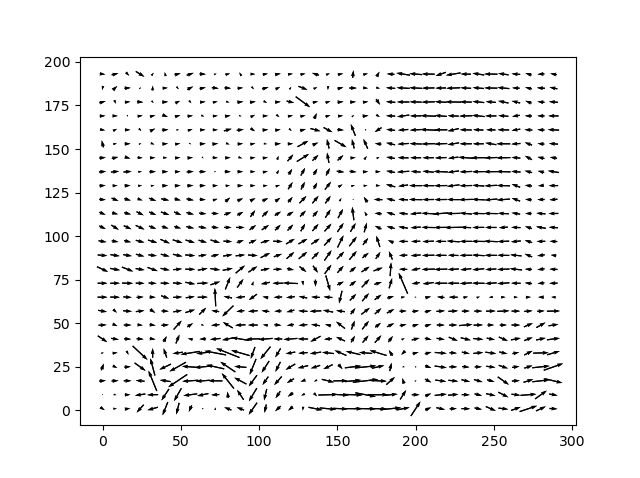
\includegraphics[height=25em]{prob4}
	\caption{Depth Map from Frankot-Chellappa Method}
	\label{fig:p4}
\end{figure*}

This algorithm is very quick, because the FFT operation makes taking a Fourier transform very efficient, and takes the place of large convolutions. It becomes infeasible if it is difficult or impossible to form the elements of the solution in Fourier space, for example if you wanted to weight individual pixels. 



\solution{5} An alternative to the algorithm in problem 4 is the Conjugate Gradient method, this has the advantage of not having to explicitly form the matrices in Fourier space. This allows us to use pixel-independent weighting, which would create a $W_X H_X \times W_X H_X$ diagonal matrix in Fourier Space. The weighting we used is 
\begin{align}
	w[n] = (\hat{n}_z[n])^2
\end{align}
and we want to use the least-squares formulation,
\begin{align}
	Z = \underset{Z}{\arg \min} \sum_n w[n](g_x[n]-(f_x*Z)[n])^2 + \sum_n w[n](g_y[n]-(f_y*Z)[n])^2 + \lambda R(Z)
\end{align}
which we can write as a quadratic equation in $Z$,
\begin{align}
	Z = \underset{Z}{\arg \min}\ \  Z^TQZ-2Z^Tb+c
\end{align}
which we can use conjugate gradient method to solve without explicitly forming the $W_X H_X \times W_X H_X$ matrix $Q$. The algorithm describes an initialization
\begin{align}
		r_0 = p_0 = b-Q*Z_0 
\end{align}
and iterative update,
\begin{align}
	\begin{split}
		\alpha_k &= \dfrac{||r_k||^2}{p_k^TQp_k}\\
		Z_{k+1} &= Z_k + \alpha_kp_k\\
		r_{k+1} &= r_k - \alpha_kQp_k\\
		\beta_k &= \dfrac{||r_{k+1}||^2}{||r_k||^2} \\
		p_{k+1} &= r_{k+1} + \beta_kp_k
	\end{split}
\end{align}
for each iteration of the algorithm $k=\{0,\ 1,\ \dots\ ,\ K\}$, returning $Z_K$, where $Z_i,\ r_i,\ p_i$ are image shaped objects and $\alpha_i,\ \beta_i$ are scalars.

From equation 35 we can see that there is no scalar component in the quadratic, and we can use a fourier transform write expressions for $b$ and $Q$,
\begin{align}
	\mathcal{F}(Q) &= F_x^TWF_x + F_y^TWF_y+\lambda F_r^TF_r \\
	\mathcal{F}(b) &= F_x^TWG_x+F_y^TWG_y
\end{align}
$b$ we can inverse transform, turning multiplication in transform space into convolutions, since $b$ is an image shaped object,
\begin{align}
	b = (g_x \times w)*\bar{f}_x + (g_y \times w)*\bar{f}_y
\end{align}
where $\times$ denotes element-wise multiplication, and $\bar{f}_i$ denotes the flipped kernel of $f_i$, which comes from the transpose of a kernel $F_i^T$ in Fourier space. $Q$, as a square matrix denotes a convolution operation, so we can formulate $Qp$ the matrix multiplication of $Q$ with a image shaped vector, $p$
\begin{align}
	Qp = ((p*f_x)\times w)*\bar{f}_x + ((p*f_y)\times w)*\bar{f}_y + \lambda((p*f_r)*f_r)
\end{align}
The result of this algorithm is shown in Figure \ref{fig:p5}. 

\begin{figure*}[!h]
	\centering
	\includegraphics[height=25em]{prob5}
	\caption{Depth Map from Conjugate Gradient Method}
	\label{fig:p5}
\end{figure*}

This algorithm is much more expensive than the Frankot-Chellappa Method, since there are $K$ iterations where you have to compute multiple convolutions across the whole image, instead of only a handful of image sized FFTs and elementwise multiplications, however it has the potential to be accurate since we are able to apply a weight to individual pixels. This can be seen in the differences between Figures \ref{fig:p4} and \ref{fig:p5}, where there are finer details in Figure \ref{fig:p5}.

%%%%%%%%%% Important, you must edit and complete the informational
%%%%%%%%%% section below. If you discussed the problem set with no
%%%%%%%%%% one, edit it to say no discussions or external resources.
\info

This problem set took approximately 20 hours of effort.

I discussed this problem set with only the instructor.

% Note that you might have to escape some special symbols in URLS like \_
I also got hints from no outside resources. 

\end{document}
